\documentclass{report}

%%%%%%%%%%%%%%%%%%%%%%%%%%%%%%%%
% PACKAGE IMPORTS
%%%%%%%%%%%%%%%%%%%%%%%%%%%%%%%%%


\usepackage[tmargin=2cm,rmargin=1in,lmargin=1in,margin=0.85in,bmargin=2cm,footskip=.2in]{geometry}
\usepackage{amsmath,amsfonts,amsthm,amssymb,mathtools}
\usepackage[varbb]{newpxmath}
\usepackage{xfrac}
\usepackage[makeroom]{cancel}
\usepackage{mathtools}
\usepackage{bookmark}
\usepackage{enumitem}
\usepackage{hyperref,theoremref}
\hypersetup{
	pdftitle={Assignment},
	colorlinks=true, linkcolor=doc!90,
	bookmarksnumbered=true,
	bookmarksopen=true
}
\usepackage[most,many,breakable]{tcolorbox}
\usepackage{xcolor}
\usepackage{varwidth}
\usepackage{varwidth}
\usepackage{etoolbox}
%\usepackage{authblk}
\usepackage{nameref}
\usepackage{multicol,array}
\usepackage{tikz-cd}
\usepackage{tikz-3dplot}
\usepackage[ruled,vlined,linesnumbered]{algorithm2e}
\usepackage{comment} % enables the use of multi-line comments (\ifx \fi) 
\usepackage{import}
\usepackage{xifthen}
\usepackage{pdfpages}
\usepackage{transparent}
\usepackage{graphicx} % <-- Added package to handle graphics
\usepackage{xcolor}
\usepackage{pgfplots}
\usepackage{minted}
\definecolor{pastelFDF7C3}{HTML}{FDF7C3}
\pgfplotsset{compat=newest}
\usepgfplotslibrary{colormaps}


\newcommand\mycommfont[1]{\footnotesize\ttfamily\textcolor{blue}{#1}}
\SetCommentSty{mycommfont}
\newcommand{\incfig}[1]{%
    \def\svgwidth{\columnwidth}
    \import{./figures/}{#1.pdf_tex}
}

\usepackage{tikzsymbols}
\renewcommand\qedsymbol{$\Laughey$}


%\usepackage{import}
%\usepackage{xifthen}
%\usepackage{pdfpages}
%\usepackage{transparent}


%%%%%%%%%%%%%%%%%%%%%%%%%%%%%%
% SELF MADE COLORS
%%%%%%%%%%%%%%%%%%%%%%%%%%%%%%



\definecolor{myg}{RGB}{56, 140, 70}
\definecolor{myb}{RGB}{45, 111, 177}
\definecolor{myr}{RGB}{199, 68, 64}
\definecolor{mytheorembg}{HTML}{F2F2F9}
\definecolor{mytheoremfr}{HTML}{00007B}
\definecolor{mylenmabg}{HTML}{FFFAF8}
\definecolor{mylenmafr}{HTML}{983b0f}
\definecolor{mypropbg}{HTML}{f2fbfc}
\definecolor{mypropfr}{HTML}{191971}
\definecolor{myexamplebg}{HTML}{F2FBF8}
\definecolor{myexamplefr}{HTML}{88D6D1}
\definecolor{myexampleti}{HTML}{2A7F7F}
\definecolor{mydefinitbg}{HTML}{E5E5FF}
\definecolor{mydefinitfr}{HTML}{3F3FA3}
\definecolor{notesgreen}{RGB}{0,162,0}
\definecolor{myp}{RGB}{197, 92, 212}
\definecolor{mygr}{HTML}{2C3338}
\definecolor{myred}{RGB}{127,0,0}
\definecolor{myyellow}{RGB}{169,121,69}
\definecolor{myexercisebg}{HTML}{F2FBF8}
\definecolor{myexercisefg}{HTML}{88D6D1}


%%%%%%%%%%%%%%%%%%%%%%%%%%%%
% TCOLORBOX SETUPS
%%%%%%%%%%%%%%%%%%%%%%%%%%%%

\setlength{\parindent}{1cm}
%================================
% THEOREM BOX
%================================

\tcbuselibrary{theorems,skins,hooks}
\newtcbtheorem[number within=section]{Theorem}{Theorem}
{%
	enhanced,
	breakable,
	colback = mytheorembg,
	frame hidden,
	boxrule = 0sp,
	borderline west = {2pt}{0pt}{mytheoremfr},
	sharp corners,
	detach title,
	before upper = \tcbtitle\par\smallskip,
	coltitle = mytheoremfr,
	fonttitle = \bfseries\sffamily,
	description font = \mdseries,
	separator sign none,
	segmentation style={solid, mytheoremfr},
}
{th}

\tcbuselibrary{theorems,skins,hooks}
\newtcbtheorem[number within=chapter]{theorem}{Theorem}
{%
	enhanced,
	breakable,
	colback = mytheorembg,
	frame hidden,
	boxrule = 0sp,
	borderline west = {2pt}{0pt}{mytheoremfr},
	sharp corners,
	detach title,
	before upper = \tcbtitle\par\smallskip,
	coltitle = mytheoremfr,
	fonttitle = \bfseries\sffamily,
	description font = \mdseries,
	separator sign none,
	segmentation style={solid, mytheoremfr},
}
{th}


\tcbuselibrary{theorems,skins,hooks}
\newtcolorbox{Theoremcon}
{%
	enhanced
	,breakable
	,colback = mytheorembg
	,frame hidden
	,boxrule = 0sp
	,borderline west = {2pt}{0pt}{mytheoremfr}
	,sharp corners
	,description font = \mdseries
	,separator sign none
}

%================================
% Corollery
%================================
\tcbuselibrary{theorems,skins,hooks}
\newtcbtheorem[number within=section]{Corollary}{Corollary}
{%
	enhanced
	,breakable
	,colback = myp!10
	,frame hidden
	,boxrule = 0sp
	,borderline west = {2pt}{0pt}{myp!85!black}
	,sharp corners
	,detach title
	,before upper = \tcbtitle\par\smallskip
	,coltitle = myp!85!black
	,fonttitle = \bfseries\sffamily
	,description font = \mdseries
	,separator sign none
	,segmentation style={solid, myp!85!black}
}
{th}
\tcbuselibrary{theorems,skins,hooks}
\newtcbtheorem[number within=chapter]{corollary}{Corollary}
{%
	enhanced
	,breakable
	,colback = myp!10
	,frame hidden
	,boxrule = 0sp
	,borderline west = {2pt}{0pt}{myp!85!black}
	,sharp corners
	,detach title
	,before upper = \tcbtitle\par\smallskip
	,coltitle = myp!85!black
	,fonttitle = \bfseries\sffamily
	,description font = \mdseries
	,separator sign none
	,segmentation style={solid, myp!85!black}
}
{th}


%================================
% LENMA
%================================

\tcbuselibrary{theorems,skins,hooks}
\newtcbtheorem[number within=section]{Lenma}{Lenma}
{%
	enhanced,
	breakable,
	colback = mylenmabg,
	frame hidden,
	boxrule = 0sp,
	borderline west = {2pt}{0pt}{mylenmafr},
	sharp corners,
	detach title,
	before upper = \tcbtitle\par\smallskip,
	coltitle = mylenmafr,
	fonttitle = \bfseries\sffamily,
	description font = \mdseries,
	separator sign none,
	segmentation style={solid, mylenmafr},
}
{th}

\tcbuselibrary{theorems,skins,hooks}
\newtcbtheorem[number within=chapter]{lenma}{Lenma}
{%
	enhanced,
	breakable,
	colback = mylenmabg,
	frame hidden,
	boxrule = 0sp,
	borderline west = {2pt}{0pt}{mylenmafr},
	sharp corners,
	detach title,
	before upper = \tcbtitle\par\smallskip,
	coltitle = mylenmafr,
	fonttitle = \bfseries\sffamily,
	description font = \mdseries,
	separator sign none,
	segmentation style={solid, mylenmafr},
}
{th}


%================================
% PROPOSITION
%================================

\tcbuselibrary{theorems,skins,hooks}
\newtcbtheorem[number within=section]{Prop}{Proposition}
{%
	enhanced,
	breakable,
	colback = mypropbg,
	frame hidden,
	boxrule = 0sp,
	borderline west = {2pt}{0pt}{mypropfr},
	sharp corners,
	detach title,
	before upper = \tcbtitle\par\smallskip,
	coltitle = mypropfr,
	fonttitle = \bfseries\sffamily,
	description font = \mdseries,
	separator sign none,
	segmentation style={solid, mypropfr},
}
{th}

\tcbuselibrary{theorems,skins,hooks}
\newtcbtheorem[number within=chapter]{prop}{Proposition}
{%
	enhanced,
	breakable,
	colback = mypropbg,
	frame hidden,
	boxrule = 0sp,
	borderline west = {2pt}{0pt}{mypropfr},
	sharp corners,
	detach title,
	before upper = \tcbtitle\par\smallskip,
	coltitle = mypropfr,
	fonttitle = \bfseries\sffamily,
	description font = \mdseries,
	separator sign none,
	segmentation style={solid, mypropfr},
}
{th}


%================================
% CLAIM
%================================

\tcbuselibrary{theorems,skins,hooks}
\newtcbtheorem[number within=section]{claim}{Claim}
{%
	enhanced
	,breakable
	,colback = myg!10
	,frame hidden
	,boxrule = 0sp
	,borderline west = {2pt}{0pt}{myg}
	,sharp corners
	,detach title
	,before upper = \tcbtitle\par\smallskip
	,coltitle = myg!85!black
	,fonttitle = \bfseries\sffamily
	,description font = \mdseries
	,separator sign none
	,segmentation style={solid, myg!85!black}
}
{th}



%================================
% Exercise
%================================

\tcbuselibrary{theorems,skins,hooks}
\newtcbtheorem[number within=section]{Exercise}{Exercise}
{%
	enhanced,
	breakable,
	colback = myexercisebg,
	frame hidden,
	boxrule = 0sp,
	borderline west = {2pt}{0pt}{myexercisefg},
	sharp corners,
	detach title,
	before upper = \tcbtitle\par\smallskip,
	coltitle = myexercisefg,
	fonttitle = \bfseries\sffamily,
	description font = \mdseries,
	separator sign none,
	segmentation style={solid, myexercisefg},
}
{th}

\tcbuselibrary{theorems,skins,hooks}
\newtcbtheorem[number within=chapter]{exercise}{Exercise}
{%
	enhanced,
	breakable,
	colback = myexercisebg,
	frame hidden,
	boxrule = 0sp,
	borderline west = {2pt}{0pt}{myexercisefg},
	sharp corners,
	detach title,
	before upper = \tcbtitle\par\smallskip,
	coltitle = myexercisefg,
	fonttitle = \bfseries\sffamily,
	description font = \mdseries,
	separator sign none,
	segmentation style={solid, myexercisefg},
}
{th}

%================================
% EXAMPLE BOX (Lighter Pastel Purple)
%================================

\definecolor{pastelExampleBg}{HTML}{70AF85} % Base pastel color
\definecolor{greenPast}{HTML}{86C8BC} % Base pastel color
\colorlet{myexamplebg}{pastelExampleBg!25!white} % Mix with white for a pastel color
\colorlet{myexamplefr}{pastelExampleBg!85!white} % Use the same mix for the frame
\colorlet{myexampleti}{greenPast!40!black} % Mix A1EEBD with black for a darker green

\newtcbtheorem[number within=section]{Example}{Example}
{%
	colback = myexamplebg
	,breakable
	,colframe = myexamplefr
	,coltitle = myexampleti
	,boxrule = 1pt
	,sharp corners
	,detach title
	,before upper=\tcbtitle\par\smallskip
	,fonttitle = \bfseries
	,description font = \mdseries
	,separator sign none
	,description delimiters parenthesis
}
{ex}

\newtcbtheorem[number within=chapter]{example}{Example}
{%
	colback = myexamplebg
	,breakable
	,colframe = myexamplefr
	,coltitle = myexampleti
	,boxrule = 1pt
	,sharp corners
	,detach title
	,before upper=\tcbtitle\par\smallskip
	,fonttitle = \bfseries
	,description font = \mdseries
	,separator sign none
	,description delimiters parenthesis
}
{ex}

%================================
% EXAMPLE BOX (Rose)
%================================

% Define the custom example box with rose image in the top-right corner
\newtcolorbox[auto counter, number within=section]{ExampleWithRose}[2][]{%
    colback=myexamplebg,  % Use the pastel version of BFF6C3 for the background
    colframe=myexamplefr, % Use the pastel version of BFF6C3 for the frame
    coltitle=myexampleti, % Use black for the title color
    fonttitle=\bfseries,
    title={Example~\thetcbcounter: #2},
    sharp corners,
    enhanced,
    overlay={
        \node[anchor=south east] at (frame.south east) {
\includegraphics[width=1.5cm]{flow.png}};
    },
    #1
}

%================================
% DEFINITION BOX
%================================

\makeatletter
\definecolor{customblue}{RGB}{198, 220, 228} % Custom blue color
\definecolor{darkblue}{RGB}{90, 120, 140} % Darker blue for text

\newtcbtheorem[number within=section]{Definition}{Definition}{enhanced,
	before skip=2mm,after skip=2mm, colback=customblue!20,colframe=customblue!80,boxrule=0.5mm,
	attach boxed title to top left={xshift=1cm,yshift*=1mm-\tcboxedtitleheight}, varwidth boxed title*=-3cm,
	boxed title style={frame code={
					\path[fill=customblue]  % Custom blue fill
					([yshift=-1mm,xshift=-1mm]frame.north west)
					arc[start angle=0,end angle=180,radius=1mm]
					([yshift=-1mm,xshift=1mm]frame.north east)
					arc[start angle=180,end angle=0,radius=1mm];
					\path[left color=customblue,right color=customblue,
						middle color=customblue!90]  % Light custom blue gradient
					([xshift=-2mm]frame.north west) -- ([xshift=2mm]frame.north east)
					[rounded corners=1mm]-- ([xshift=1mm,yshift=-1mm]frame.north east)
					-- (frame.south east) -- (frame.south west)
					-- ([xshift=-1mm,yshift=-1mm]frame.north west)
					[sharp corners]-- cycle;
				},interior engine=empty,
		},
	fonttitle=\bfseries\color{darkblue}, % Darker blue for the title text
	coltitle=darkblue, % Darker blue for the box title
	colbacktitle=customblue!80, % Background for the title
	title={#2},#1}{def}

\newtcbtheorem[number within=chapter]{definition}{Definition}{enhanced,
	before skip=2mm,after skip=2mm, colback=customblue!20,colframe=customblue!80,boxrule=0.5mm,
	attach boxed title to top left={xshift=1cm,yshift*=1mm-\tcboxedtitleheight}, varwidth boxed title*=-3cm,
	boxed title style={frame code={
					\path[fill=customblue]  % Custom blue fill
					([yshift=-1mm,xshift=-1mm]frame.north west)
					arc[start angle=0,end angle=180,radius=1mm]
					([yshift=-1mm,xshift=1mm]frame.north east)
					arc[start angle=180,end angle=0,radius=1mm];
					\path[left color=customblue,right color=customblue,
						middle color=customblue!90]  % Light custom blue gradient
					([xshift=-2mm]frame.north west) -- ([xshift=2mm]frame.north east)
					[rounded corners=1mm]-- ([xshift=1mm,yshift=-1mm]frame.north east)
					-- (frame.south east) -- (frame.south west)
					-- ([xshift=-1mm,yshift=-1mm]frame.north west)
					[sharp corners]-- cycle;
				},interior engine=empty,
		},
	fonttitle=\bfseries\color{darkblue}, % Darker blue for the title text
	coltitle=darkblue, % Darker blue for the box title
	colbacktitle=customblue!80, % Background for the title
	title={#2},#1}{def}
\makeatother

%================================
% DEFINITION BOX WITH IMAGE IN BOTTOM-RIGHT
%================================

%================================
% DEFINITION BOX WITH IMAGE IN BOTTOM-RIGHT
%================================

\makeatletter
\definecolor{customblue}{RGB}{198, 234, 245} % Custom blue color
\definecolor{darkblue}{RGB}{90, 120, 140} % Darker blue for text

\newtcbtheorem[number within=section]{DefinitionWithImage}{Definition}{enhanced,
	before skip=2mm,
	after skip=2mm, 
	colback=customblue!40, % Use custom blue with 20% intensity for background
	colframe=customblue!80!black, % Use custom blue with some black for the frame
	boxrule=0.5mm,
	attach boxed title to top left={xshift=1cm,yshift*=1mm-\tcboxedtitleheight}, 
	varwidth boxed title*=-3cm,
	boxed title style={frame code={
					\path[fill=customblue]  % Custom blue fill
					([yshift=-1mm,xshift=-1mm]frame.north west)
					arc[start angle=0,end angle=180,radius=1mm]
					([yshift=-1mm,xshift=1mm]frame.north east)
					arc[start angle=180,end angle=0,radius=1mm];
					\path[left color=customblue,right color=customblue,
						middle color=customblue!90]  % Light custom blue gradient
					([xshift=-2mm]frame.north west) -- ([xshift=2mm]frame.north east)
					[rounded corners=1mm]-- ([xshift=1mm,yshift=-1mm]frame.north east)
					-- (frame.south east) -- (frame.south west)
					-- ([xshift=-1mm,yshift=-1mm]frame.north west)
					[sharp corners]-- cycle;
				},interior engine=empty,
		},
	fonttitle=\bfseries\color{darkblue}, % Darker blue for the title text
	coltitle=darkblue, % Darker blue for the box title
	colbacktitle=customblue!80, % Background for the title
	title={#2},
	overlay unbroken and last={
		\node[anchor=south east,xshift=-2mm,yshift=2mm] at (frame.south east) {
\includegraphics[width=1 cm]{slime.png}};
	} % Adjust the path and size to your needs
}{def}
\makeatother

%================================
% Solution BOX (Pastel Light Blue)
%================================

\makeatletter
\definecolor{pastelpink}{HTML}{FFE3ED} % Define pastel pink using the hex code #FFE3ED

\newtcbtheorem{question}{Question}{enhanced,
	breakable,
	colback=pastelpink!60, % Use pastel pink for the background with 60% intensity
	colframe=pastelpink!90!black, % Use pastel pink with a bit of black for the frame
	attach boxed title to top left={yshift*=-\tcboxedtitleheight},
	fonttitle=\bfseries,
	title={#2},
	boxed title size=title,
	boxed title style={%
			sharp corners,
			rounded corners=northwest,
			colback=tcbcolframe,
			boxrule=0pt,
		},
	underlay boxed title={%
			\path[fill=tcbcolframe] (title.south west)--(title.south east)
			to[out=0, in=180] ([xshift=5mm]title.east)--
			(title.center-|frame.east)
			[rounded corners=\kvtcb@arc] |-
			(frame.north) -| cycle;
		},
	#1
}{def}
\makeatother


% SOLUTION BOX
%================================

\makeatletter
\newtcolorbox{solution}{enhanced,
	breakable,
	colback=white,
	colframe=myg!80!black,
	attach boxed title to top left={yshift*=-\tcboxedtitleheight},
	title=Solution,
	boxed title size=title,
	boxed title style={%
			sharp corners,
			rounded corners=northwest,
			colback=tcbcolframe,
			boxrule=0pt,
		},
	underlay boxed title={%
			\path[fill=tcbcolframe] (title.south west)--(title.south east)
			to[out=0, in=180] ([xshift=5mm]title.east)--
			(title.center-|frame.east)
			[rounded corners=\kvtcb@arc] |-
			(frame.north) -| cycle;
		},
}
\makeatother

%================================
% Question BOX
%================================

\makeatletter
\newtcbtheorem{qstion}{Question}{enhanced,
	breakable,
	colback=white,
	colframe=mygr,
	attach boxed title to top left={yshift*=-\tcboxedtitleheight},
	fonttitle=\bfseries,
	title={#2},
	boxed title size=title,
	boxed title style={%
			sharp corners,
			rounded corners=northwest,
			colback=tcbcolframe,
			boxrule=0pt,
		},
	underlay boxed title={%
			\path[fill=tcbcolframe] (title.south west)--(title.south east)
			to[out=0, in=180] ([xshift=5mm]title.east)--
			(title.center-|frame.east)
			[rounded corners=\kvtcb@arc] |-
			(frame.north) -| cycle;
		},
	#1
}{def}
\makeatother

\newtcbtheorem[number within=chapter]{wconc}{Wrong Concept}{
	breakable,
	enhanced,
	colback=white,
	colframe=myr,
	arc=0pt,
	outer arc=0pt,
	fonttitle=\bfseries\sffamily\large,
	colbacktitle=myr,
	attach boxed title to top left={},
	boxed title style={
			enhanced,
			skin=enhancedfirst jigsaw,
			arc=3pt,
			bottom=0pt,
			interior style={fill=myr}
		},
	#1
}{def}



%================================
% NOTE BOX (Pastel Pink)
%================================

\usetikzlibrary{arrows,calc,shadows.blur}
\tcbuselibrary{skins}
\definecolor{pastelpink}{HTML}{FFE3ED} % Define pastel pink using the hex code #FFE3ED

\newtcolorbox{note}[1][]{%
    enhanced jigsaw,
    colback=pastelpink, % Use pastel pink for the background
    colframe=pastelpink, % Use pastel pink for the frame
    size=small,
    boxrule=1pt,
    title=\textbf{Note:-},
    halign title=flush center,
    coltitle=black,
    breakable,
    drop shadow=black!50!white,
    attach boxed title to top left={xshift=1cm,yshift=-\tcboxedtitleheight/2,yshifttext=-\tcboxedtitleheight/2},
    minipage boxed title=1.5cm,
    boxed title style={%
            colback=white,
            size=fbox,
            boxrule=1pt,
            boxsep=2pt,
            underlay={%
                    \coordinate (dotA) at ($(interior.west) + (-0.5pt,0)$);
                    \coordinate (dotB) at ($(interior.east) + (0.5pt,0)$);
                    \begin{scope}
                        \clip (interior.north west) rectangle ([xshift=3ex]interior.east);
                        \filldraw [white, blur shadow={shadow opacity=60, shadow yshift=-.75ex}, rounded corners=2pt] (interior.north west) rectangle (interior.south east);
                    \end{scope}
                    \begin{scope}[pastelpink]
                        \fill (dotA) circle (2pt);
                        \fill (dotB) circle (2pt);
                    \end{scope}
                },
        },
    #1,
}

%================================
% NOTE BOX (Pastel Pink with Image in Bottom-Left)
%================================
\newtcolorbox{noteWithImage}[1][]{%
    enhanced jigsaw,
    colback=pastelFDF7C3!70!white, % Mix pastelFDF7C3 with white to lighten the color
    colframe=pastelFDF7C3!80!white, % Mix pastelFDF7C3 with white for the frame
    size=small,
    boxrule=1pt,
    title=\textbf{Note:-},
    halign title=flush center,
    coltitle=black,
    breakable,
    drop shadow=black!50!white,
    attach boxed title to top left={xshift=1cm,yshift=-\tcboxedtitleheight/2,yshifttext=-\tcboxedtitleheight/2},
    minipage boxed title=1.5cm,
    boxed title style={%
            colback=white,
            size=fbox,
            boxrule=1pt,
            boxsep=2pt,
            underlay={%
                    \coordinate (dotA) at ($(interior.west) + (-0.5pt,0)$);
                    \coordinate (dotB) at ($(interior.east) + (0.5pt,0)$);
                    \begin{scope}
                        \clip (interior.north west) rectangle ([xshift=3ex]interior.east);
                        \filldraw [white, blur shadow={shadow opacity=60, shadow yshift=-.75ex}, rounded corners=2pt] (interior.north west) rectangle (interior.south east);
                    \end{scope}
                    \begin{scope}[pastelFDF7C3!80!white]
                        \fill (dotA) circle (2pt);
                        \fill (dotB) circle (2pt);
                    \end{scope}
                },
        },
    overlay unbroken and last={
        \node[anchor=south east,xshift=-2mm,yshift=1mm] at (frame.south east) {
\includegraphics[width=1cm]{lot.png}};
    }, % Replace 'rose.png' with the path to your image
    #1,
}


%%%%%%%%%%%%%%%%%%%%%%%%%%%%%%
% SELF MADE COMMANDS
%%%%%%%%%%%%%%%%%%%%%%%%%%%%%%


\newcommand{\thm}[2]{\begin{Theorem}{#1}{}#2\end{Theorem}}
\newcommand{\cor}[2]{\begin{Corollary}{#1}{}#2\end{Corollary}}
\newcommand{\mlenma}[2]{\begin{Lenma}{#1}{}#2\end{Lenma}}
\newcommand{\mprop}[2]{\begin{Prop}{#1}{}#2\end{Prop}}
\newcommand{\clm}[3]{\begin{claim}{#1}{#2}#3\end{claim}}
\newcommand{\wc}[2]{\begin{wconc}{#1}{}\setlength{\parindent}{1cm}#2\end{wconc}}
\newcommand{\thmcon}[1]{\begin{Theoremcon}{#1}\end{Theoremcon}}
\newcommand{\exer}[2]{\begin{Exercise}{#1}{}#2\end{Exercise}}
\newcommand{\ex}[2]{\begin{Example}{#1}{}#2\end{Example}}
\newcommand{\dfn}[2]{\begin{Definition}[colbacktitle=red!75!black]{#1}{}#2\end{Definition}}
\newcommand{\dfnc}[2]{\begin{definition}[colbacktitle=red!75!black]{#1}{}#2\end{definition}}
\newcommand{\qs}[2]{\begin{question}{#1}{}#2\end{question}}
\newcommand{\pf}[2]{\begin{myproof}[#1]#2\end{myproof}}
\newcommand{\nt}[1]{\begin{note}#1\end{note}}
\newcommand{\insertpng}[2][1]{\begin{center} \includegraphics[scale=#1]{#2} \end{center}} % <-- New command for PNG insertion

\newcommand{\defrose}[2]{%
    \begin{DefinitionWithImage}{#1}%
        #2%
    \end{DefinitionWithImage}%
}

\newcommand{\exrose}[2]{%
    \begin{ExampleWithRose}{#1}%
        #2%
    \end{ExampleWithRose}%
}

\newcommand{\ntimg}[2][]{%
    \begin{noteWithImage}[#1]%
        #2%
    \end{noteWithImage}%
}

\newcommand*\circled[1]{\tikz[baseline=(char.base)]{
		\node[shape=circle,draw,inner sep=1pt] (char) {#1};}}
\newcommand\getcurrentref[1]{%
	\ifnumequal{\value{#1}}{0}
	{??}
	{\the\value{#1}}%
}
\newcommand{\getCurrentSectionNumber}{\getcurrentref{section}}
\newenvironment{myproof}[1][\proofname]{%
	\proof[\bfseries #1: ]%
}{\endproof}

\newcommand{\mclm}[2]{\begin{myclaim}[#1]#2\end{myclaim}}
\newenvironment{myclaim}[1][\claimname]{\proof[\bfseries #1: ]}{}

\newcounter{mylabelcounter}

\makeatletter
\newcommand{\setword}[2]{%
	\phantomsection
	#1\def\@currentlabel{\unexpanded{#1}}\label{#2}%
}
\makeatother




\tikzset{
	symbol/.style={
			draw=none,
			every to/.append style={
					edge node={node [sloped, allow upside down, auto=false]{$#1$}}}
		}
}


% deliminators
\DeclarePairedDelimiter{\abs}{\lvert}{\rvert}
\DeclarePairedDelimiter{\norm}{\lVert}{\rVert}

\DeclarePairedDelimiter{\ceil}{\lceil}{\rceil}
\DeclarePairedDelimiter{\floor}{\lfloor}{\rfloor}
\DeclarePairedDelimiter{\round}{\lfloor}{\rceil}

\newsavebox\diffdbox
\newcommand{\slantedromand}{{\mathpalette\makesl{d}}}
\newcommand{\makesl}[2]{%
\begingroup
\sbox{\diffdbox}{$\mathsurround=0pt#1\mathrm{#2}$}%
\pdfsave
\pdfsetmatrix{1 0 0.2 1}%
\rlap{\usebox{\diffdbox}}%
\pdfrestore
\hskip\wd\diffdbox
\endgroup
}
\newcommand{\dd}[1][]{\ensuremath{\mathop{}\!\ifstrempty{#1}{%
\slantedromand\@ifnextchar^{\hspace{0.2ex}}{\hspace{0.1ex}}}%
{\slantedromand\hspace{0.2ex}^{#1}}}}
\ProvideDocumentCommand\dv{o m g}{%
  \ensuremath{%
    \IfValueTF{#3}{%
      \IfNoValueTF{#1}{%
        \frac{\dd #2}{\dd #3}%
      }{%
        \frac{\dd^{#1} #2}{\dd #3^{#1}}%
      }%
    }{%
      \IfNoValueTF{#1}{%
        \frac{\dd}{\dd #2}%
      }{%
        \frac{\dd^{#1}}{\dd #2^{#1}}%
      }%
    }%
  }%
}
\providecommand*{\pdv}[3][]{\frac{\partial^{#1}#2}{\partial#3^{#1}}}
%  - others
\DeclareMathOperator{\Lap}{\mathcal{L}}
\DeclareMathOperator{\Var}{Var} % varience
\DeclareMathOperator{\Cov}{Cov} % covarience
\DeclareMathOperator{\E}{E} % expected

% Since the amsthm package isn't loaded

% I prefer the slanted \leq
\let\oldleq\leq % save them in case they're every wanted
\let\oldgeq\geq
\renewcommand{\leq}{\leqslant}
\renewcommand{\geq}{\geqslant}

% % redefine matrix env to allow for alignment, use r as default
% \renewcommand*\env@matrix[1][r]{\hskip -\arraycolsep
%     \let\@ifnextchar\new@ifnextchar
%     \array{*\c@MaxMatrixCols #1}}


%\usepackage{framed}
%\usepackage{titletoc}
%\usepackage{etoolbox}
%\usepackage{lmodern}


%\patchcmd{\tableofcontents}{\contentsname}{\sffamily\contentsname}{}{}

%\renewenvironment{leftbar}
%{\def\FrameCommand{\hspace{6em}%
%		{\color{myyellow}\vrule width 2pt depth 6pt}\hspace{1em}}%
%	\MakeFramed{\parshape 1 0cm \dimexpr\textwidth-6em\relax\FrameRestore}\vskip2pt%
%}
%{\endMakeFramed}

%\titlecontents{chapter}
%[0em]{\vspace*{2\baselineskip}}
%{\parbox{4.5em}{%
%		\hfill\Huge\sffamily\bfseries\color{myred}\thecontentspage}%
%	\vspace*{-2.3\baselineskip}\leftbar\textsc{\small\chaptername~\thecontentslabel}\\\sffamily}
%{}{\endleftbar}
%\titlecontents{section}
%[8.4em]
%{\sffamily\contentslabel{3em}}{}{}
%{\hspace{0.5em}\nobreak\itshape\color{myred}\contentspage}
%\titlecontents{subsection}
%[8.4em]
%{\sffamily\contentslabel{3em}}{}{}  
%{\hspace{0.5em}\nobreak\itshape\color{myred}\contentspage}



%%%%%%%%%%%%%%%%%%%%%%%%%%%%%%%%%%%%%%%%%%%
% TABLE OF CONTENTS
%%%%%%%%%%%%%%%%%%%%%%%%%%%%%%%%%%%%%%%%%%%

\usepackage{tikz}
\definecolor{doc}{HTML}{AD6989} % Define the new color using the hex code #AD6989
\usepackage{titletoc}
\contentsmargin{0cm}
\titlecontents{chapter}[3.7pc]
{\addvspace{30pt}%
	\begin{tikzpicture}[remember picture, overlay]%
		\draw[fill=doc!60,draw=doc!60] (-7,-.1) rectangle (-0.9,.5);%
		\pgftext[left,x=-3.5cm,y=0.2cm]{\color{white}\Large\sc\bfseries Chapter\ \thecontentslabel};%
	\end{tikzpicture}\color{doc!60}\large\sc\bfseries}%
{}
{}
{\;\titlerule\;\large\sc\bfseries Page \thecontentspage
	\begin{tikzpicture}[remember picture, overlay]
		\draw[fill=doc!60,draw=doc!60] (2pt,0) rectangle (4,0.1pt);
	\end{tikzpicture}}%
\titlecontents{section}[3.7pc]
{\addvspace{2pt}}
{\contentslabel[\thecontentslabel]{2pc}}
{}
{\hfill\small \thecontentspage}
[]
\titlecontents*{subsection}[3.7pc]
{\addvspace{-1pt}\small}
{}
{}
{\ --- \small\thecontentspage}
[ \textbullet\ ][]

\makeatletter
\renewcommand{\tableofcontents}{%
	\chapter*{%
	  \vspace*{-20\p@}%
	  \begin{tikzpicture}[remember picture, overlay]%
		  \pgftext[right,x=15cm,y=0.2cm]{\color{doc!60}\Huge\sc\bfseries \contentsname};%
		  \draw[fill=doc!60,draw=doc!60] (13,-.75) rectangle (20,1);%
		  \clip (13,-.75) rectangle (20,1);
		  \pgftext[right,x=15cm,y=0.2cm]{\color{white}\Huge\sc\bfseries \contentsname};%
	  \end{tikzpicture}}%
	\@starttoc{toc}}
\makeatother

%From M275 "Topology" at SJSU
\newcommand{\id}{\mathrm{id}}
\newcommand{\taking}[1]{\xrightarrow{#1}}
\newcommand{\inv}{^{-1}}

%From M170 "Introduction to Graph Theory" at SJSU
\DeclareMathOperator{\diam}{diam}
\DeclareMathOperator{\ord}{ord}
\newcommand{\defeq}{\overset{\mathrm{def}}{=}}

%From the USAMO .tex files
\newcommand{\ts}{\textsuperscript}
\newcommand{\dg}{^\circ}
\newcommand{\ii}{\item}

% % From Math 55 and Math 145 at Harvard
% \newenvironment{subproof}[1][Proof]{%
% \begin{proof}[#1] \renewcommand{\qedsymbol}{$\blacksquare$}}%
% {\end{proof}}

\newcommand{\liff}{\leftrightarrow}
\newcommand{\lthen}{\rightarrow}
\newcommand{\opname}{\operatorname}
\newcommand{\surjto}{\twoheadrightarrow}
\newcommand{\injto}{\hookrightarrow}
\newcommand{\On}{\mathrm{On}} % ordinals
\DeclareMathOperator{\img}{im} % Image
\DeclareMathOperator{\Img}{Im} % Image
\DeclareMathOperator{\coker}{coker} % Cokernel
\DeclareMathOperator{\Coker}{Coker} % Cokernel
\DeclareMathOperator{\Ker}{Ker} % Kernel
\DeclareMathOperator{\rank}{rank}
\DeclareMathOperator{\Spec}{Spec} % spectrum
\DeclareMathOperator{\Tr}{Tr} % trace
\DeclareMathOperator{\pr}{pr} % projection
\DeclareMathOperator{\ext}{ext} % extension
\DeclareMathOperator{\pred}{pred} % predecessor
\DeclareMathOperator{\dom}{dom} % domain
\DeclareMathOperator{\ran}{ran} % range
\DeclareMathOperator{\Hom}{Hom} % homomorphism
\DeclareMathOperator{\Mor}{Mor} % morphisms
\DeclareMathOperator{\End}{End} % endomorphism

\newcommand{\eps}{\epsilon}
\newcommand{\veps}{\varepsilon}
\newcommand{\ol}{\overline}
\newcommand{\ul}{\underline}
\newcommand{\wt}{\widetilde}
\newcommand{\wh}{\widehat}
\newcommand{\vocab}[1]{\textbf{\color{blue} #1}}
\providecommand{\half}{\frac{1}{2}}
\newcommand{\dang}{\measuredangle} %% Directed angle
\newcommand{\ray}[1]{\overrightarrow{#1}}
\newcommand{\seg}[1]{\overline{#1}}
\newcommand{\arc}[1]{\wideparen{#1}}
\DeclareMathOperator{\cis}{cis}
\DeclareMathOperator*{\lcm}{lcm}
\DeclareMathOperator*{\argmin}{arg min}
\DeclareMathOperator*{\argmax}{arg max}
\newcommand{\cycsum}{\sum_{\mathrm{cyc}}}
\newcommand{\symsum}{\sum_{\mathrm{sym}}}
\newcommand{\cycprod}{\prod_{\mathrm{cyc}}}
\newcommand{\symprod}{\prod_{\mathrm{sym}}}
\newcommand{\Qed}{\begin{flushright}\qed\end{flushright}}
\newcommand{\parinn}{\setlength{\parindent}{1cm}}
\newcommand{\parinf}{\setlength{\parindent}{0cm}}
% \newcommand{\norm}{\|\cdot\|}
\newcommand{\inorm}{\norm_{\infty}}
\newcommand{\opensets}{\{V_{\alpha}\}_{\alpha\in I}}
\newcommand{\oset}{V_{\alpha}}
\newcommand{\opset}[1]{V_{\alpha_{#1}}}
\newcommand{\lub}{\text{lub}}
\newcommand{\del}[2]{\frac{\partial #1}{\partial #2}}
\newcommand{\Del}[3]{\frac{\partial^{#1} #2}{\partial^{#1} #3}}
\newcommand{\deld}[2]{\dfrac{\partial #1}{\partial #2}}
\newcommand{\Deld}[3]{\dfrac{\partial^{#1} #2}{\partial^{#1} #3}}
\newcommand{\lm}{\lambda}
\newcommand{\uin}{\mathbin{\rotatebox[origin=c]{90}{$\in$}}}
\newcommand{\usubset}{\mathbin{\rotatebox[origin=c]{90}{$\subset$}}}
\newcommand{\lt}{\left}
\newcommand{\rt}{\right}
\newcommand{\bs}[1]{\boldsymbol{#1}}
\newcommand{\exs}{\exists}
\newcommand{\st}{\strut}
\newcommand{\dps}[1]{\displaystyle{#1}}

\newcommand{\sol}{\setlength{\parindent}{0cm}\textbf{\textit{Solution:}}\setlength{\parindent}{1cm} }
\newcommand{\solve}[1]{\setlength{\parindent}{0cm}\textbf{\textit{Solution: }}\setlength{\parindent}{1cm}#1 \Qed}

% Things Lie
\newcommand{\kb}{\mathfrak b}
\newcommand{\kg}{\mathfrak g}
\newcommand{\kh}{\mathfrak h}
\newcommand{\kn}{\mathfrak n}
\newcommand{\ku}{\mathfrak u}
\newcommand{\kz}{\mathfrak z}
\DeclareMathOperator{\Ext}{Ext} % Ext functor
\DeclareMathOperator{\Tor}{Tor} % Tor functor
\newcommand{\gl}{\opname{\mathfrak{gl}}} % frak gl group
\renewcommand{\sl}{\opname{\mathfrak{sl}}} % frak sl group chktex 6

% More script letters etc.
\newcommand{\SA}{\mathcal A}
\newcommand{\SB}{\mathcal B}
\newcommand{\SC}{\mathcal C}
\newcommand{\SF}{\mathcal F}
\newcommand{\SG}{\mathcal G}
\newcommand{\SH}{\mathcal H}
\newcommand{\OO}{\mathcal O}

\newcommand{\SCA}{\mathscr A}
\newcommand{\SCB}{\mathscr B}
\newcommand{\SCC}{\mathscr C}
\newcommand{\SCD}{\mathscr D}
\newcommand{\SCE}{\mathscr E}
\newcommand{\SCF}{\mathscr F}
\newcommand{\SCG}{\mathscr G}
\newcommand{\SCH}{\mathscr H}

% Mathfrak primes
\newcommand{\km}{\mathfrak m}
\newcommand{\kp}{\mathfrak p}
\newcommand{\kq}{\mathfrak q}

% number sets
\newcommand{\RR}[1][]{\ensuremath{\ifstrempty{#1}{\mathbb{R}}{\mathbb{R}^{#1}}}}
\newcommand{\NN}[1][]{\ensuremath{\ifstrempty{#1}{\mathbb{N}}{\mathbb{N}^{#1}}}}
\newcommand{\ZZ}[1][]{\ensuremath{\ifstrempty{#1}{\mathbb{Z}}{\mathbb{Z}^{#1}}}}
\newcommand{\QQ}[1][]{\ensuremath{\ifstrempty{#1}{\mathbb{Q}}{\mathbb{Q}^{#1}}}}
\newcommand{\CC}[1][]{\ensuremath{\ifstrempty{#1}{\mathbb{C}}{\mathbb{C}^{#1}}}}
\newcommand{\PP}[1][]{\ensuremath{\ifstrempty{#1}{\mathbb{P}}{\mathbb{P}^{#1}}}}
\newcommand{\HH}[1][]{\ensuremath{\ifstrempty{#1}{\mathbb{H}}{\mathbb{H}^{#1}}}}
\newcommand{\FF}[1][]{\ensuremath{\ifstrempty{#1}{\mathbb{F}}{\mathbb{F}^{#1}}}}
% expected value
\newcommand{\EE}{\ensuremath{\mathbb{E}}}
\newcommand{\charin}{\text{ char }}
\DeclareMathOperator{\sign}{sign}
\DeclareMathOperator{\Aut}{Aut}
\DeclareMathOperator{\Inn}{Inn}
\DeclareMathOperator{\Syl}{Syl}
\DeclareMathOperator{\Gal}{Gal}
\DeclareMathOperator{\GL}{GL} % General linear group
\DeclareMathOperator{\SL}{SL} % Special linear group

%---------------------------------------
% BlackBoard Math Fonts :-
%---------------------------------------

%Captital Letters
\newcommand{\bbA}{\mathbb{A}}	\newcommand{\bbB}{\mathbb{B}}
\newcommand{\bbC}{\mathbb{C}}	\newcommand{\bbD}{\mathbb{D}}
\newcommand{\bbE}{\mathbb{E}}	\newcommand{\bbF}{\mathbb{F}}
\newcommand{\bbG}{\mathbb{G}}	\newcommand{\bbH}{\mathbb{H}}
\newcommand{\bbI}{\mathbb{I}}	\newcommand{\bbJ}{\mathbb{J}}
\newcommand{\bbK}{\mathbb{K}}	\newcommand{\bbL}{\mathbb{L}}
\newcommand{\bbM}{\mathbb{M}}	\newcommand{\bbN}{\mathbb{N}}
\newcommand{\bbO}{\mathbb{O}}	\newcommand{\bbP}{\mathbb{P}}
\newcommand{\bbQ}{\mathbb{Q}}	\newcommand{\bbR}{\mathbb{R}}
\newcommand{\bbS}{\mathbb{S}}	\newcommand{\bbT}{\mathbb{T}}
\newcommand{\bbU}{\mathbb{U}}	\newcommand{\bbV}{\mathbb{V}}
\newcommand{\bbW}{\mathbb{W}}	\newcommand{\bbX}{\mathbb{X}}
\newcommand{\bbY}{\mathbb{Y}}	\newcommand{\bbZ}{\mathbb{Z}}

%---------------------------------------
% MathCal Fonts :-
%---------------------------------------

%Captital Letters
\newcommand{\mcA}{\mathcal{A}}	\newcommand{\mcB}{\mathcal{B}}
\newcommand{\mcC}{\mathcal{C}}	\newcommand{\mcD}{\mathcal{D}}
\newcommand{\mcE}{\mathcal{E}}	\newcommand{\mcF}{\mathcal{F}}
\newcommand{\mcG}{\mathcal{G}}	\newcommand{\mcH}{\mathcal{H}}
\newcommand{\mcI}{\mathcal{I}}	\newcommand{\mcJ}{\mathcal{J}}
\newcommand{\mcK}{\mathcal{K}}	\newcommand{\mcL}{\mathcal{L}}
\newcommand{\mcM}{\mathcal{M}}	\newcommand{\mcN}{\mathcal{N}}
\newcommand{\mcO}{\mathcal{O}}	\newcommand{\mcP}{\mathcal{P}}
\newcommand{\mcQ}{\mathcal{Q}}	\newcommand{\mcR}{\mathcal{R}}
\newcommand{\mcS}{\mathcal{S}}	\newcommand{\mcT}{\mathcal{T}}
\newcommand{\mcU}{\mathcal{U}}	\newcommand{\mcV}{\mathcal{V}}
\newcommand{\mcW}{\mathcal{W}}	\newcommand{\mcX}{\mathcal{X}}
\newcommand{\mcY}{\mathcal{Y}}	\newcommand{\mcZ}{\mathcal{Z}}


%---------------------------------------
% Bold Math Fonts :-
%---------------------------------------

%Captital Letters
\newcommand{\bmA}{\boldsymbol{A}}	\newcommand{\bmB}{\boldsymbol{B}}
\newcommand{\bmC}{\boldsymbol{C}}	\newcommand{\bmD}{\boldsymbol{D}}
\newcommand{\bmE}{\boldsymbol{E}}	\newcommand{\bmF}{\boldsymbol{F}}
\newcommand{\bmG}{\boldsymbol{G}}	\newcommand{\bmH}{\boldsymbol{H}}
\newcommand{\bmI}{\boldsymbol{I}}	\newcommand{\bmJ}{\boldsymbol{J}}
\newcommand{\bmK}{\boldsymbol{K}}	\newcommand{\bmL}{\boldsymbol{L}}
\newcommand{\bmM}{\boldsymbol{M}}	\newcommand{\bmN}{\boldsymbol{N}}
\newcommand{\bmO}{\boldsymbol{O}}	\newcommand{\bmP}{\boldsymbol{P}}
\newcommand{\bmQ}{\boldsymbol{Q}}	\newcommand{\bmR}{\boldsymbol{R}}
\newcommand{\bmS}{\boldsymbol{S}}	\newcommand{\bmT}{\boldsymbol{T}}
\newcommand{\bmU}{\boldsymbol{U}}	\newcommand{\bmV}{\boldsymbol{V}}
\newcommand{\bmW}{\boldsymbol{W}}	\newcommand{\bmX}{\boldsymbol{X}}
\newcommand{\bmY}{\boldsymbol{Y}}	\newcommand{\bmZ}{\boldsymbol{Z}}
%Small Letters
\newcommand{\bma}{\boldsymbol{a}}	\newcommand{\bmb}{\boldsymbol{b}}
\newcommand{\bmc}{\boldsymbol{c}}	\newcommand{\bmd}{\boldsymbol{d}}
\newcommand{\bme}{\boldsymbol{e}}	\newcommand{\bmf}{\boldsymbol{f}}
\newcommand{\bmg}{\boldsymbol{g}}	\newcommand{\bmh}{\boldsymbol{h}}
\newcommand{\bmi}{\boldsymbol{i}}	\newcommand{\bmj}{\boldsymbol{j}}
\newcommand{\bmk}{\boldsymbol{k}}	\newcommand{\bml}{\boldsymbol{l}}
\newcommand{\bmm}{\boldsymbol{m}}	\newcommand{\bmn}{\boldsymbol{n}}
\newcommand{\bmo}{\boldsymbol{o}}	\newcommand{\bmp}{\boldsymbol{p}}
\newcommand{\bmq}{\boldsymbol{q}}	\newcommand{\bmr}{\boldsymbol{r}}
\newcommand{\bms}{\boldsymbol{s}}	\newcommand{\bmt}{\boldsymbol{t}}
\newcommand{\bmu}{\boldsymbol{u}}	\newcommand{\bmv}{\boldsymbol{v}}
\newcommand{\bmw}{\boldsymbol{w}}	\newcommand{\bmx}{\boldsymbol{x}}
\newcommand{\bmy}{\boldsymbol{y}}	\newcommand{\bmz}{\boldsymbol{z}}

%---------------------------------------
% Scr Math Fonts :-
%---------------------------------------

\newcommand{\sA}{{\mathscr{A}}}   \newcommand{\sB}{{\mathscr{B}}}
\newcommand{\sC}{{\mathscr{C}}}   \newcommand{\sD}{{\mathscr{D}}}
\newcommand{\sE}{{\mathscr{E}}}   \newcommand{\sF}{{\mathscr{F}}}
\newcommand{\sG}{{\mathscr{G}}}   \newcommand{\sH}{{\mathscr{H}}}
\newcommand{\sI}{{\mathscr{I}}}   \newcommand{\sJ}{{\mathscr{J}}}
\newcommand{\sK}{{\mathscr{K}}}   \newcommand{\sL}{{\mathscr{L}}}
\newcommand{\sM}{{\mathscr{M}}}   \newcommand{\sN}{{\mathscr{N}}}
\newcommand{\sO}{{\mathscr{O}}}   \newcommand{\sP}{{\mathscr{P}}}
\newcommand{\sQ}{{\mathscr{Q}}}   \newcommand{\sR}{{\mathscr{R}}}
\newcommand{\sS}{{\mathscr{S}}}   \newcommand{\sT}{{\mathscr{T}}}
\newcommand{\sU}{{\mathscr{U}}}   \newcommand{\sV}{{\mathscr{V}}}
\newcommand{\sW}{{\mathscr{W}}}   \newcommand{\sX}{{\mathscr{X}}}
\newcommand{\sY}{{\mathscr{Y}}}   \newcommand{\sZ}{{\mathscr{Z}}}


%---------------------------------------
% Math Fraktur Font
%---------------------------------------

%Captital Letters
\newcommand{\mfA}{\mathfrak{A}}	\newcommand{\mfB}{\mathfrak{B}}
\newcommand{\mfC}{\mathfrak{C}}	\newcommand{\mfD}{\mathfrak{D}}
\newcommand{\mfE}{\mathfrak{E}}	\newcommand{\mfF}{\mathfrak{F}}
\newcommand{\mfG}{\mathfrak{G}}	\newcommand{\mfH}{\mathfrak{H}}
\newcommand{\mfI}{\mathfrak{I}}	\newcommand{\mfJ}{\mathfrak{J}}
\newcommand{\mfK}{\mathfrak{K}}	\newcommand{\mfL}{\mathfrak{L}}
\newcommand{\mfM}{\mathfrak{M}}	\newcommand{\mfN}{\mathfrak{N}}
\newcommand{\mfO}{\mathfrak{O}}	\newcommand{\mfP}{\mathfrak{P}}
\newcommand{\mfQ}{\mathfrak{Q}}	\newcommand{\mfR}{\mathfrak{R}}
\newcommand{\mfS}{\mathfrak{S}}	\newcommand{\mfT}{\mathfrak{T}}
\newcommand{\mfU}{\mathfrak{U}}	\newcommand{\mfV}{\mathfrak{V}}
\newcommand{\mfW}{\mathfrak{W}}	\newcommand{\mfX}{\mathfrak{X}}
\newcommand{\mfY}{\mathfrak{Y}}	\newcommand{\mfZ}{\mathfrak{Z}}
%Small Letters
\newcommand{\mfa}{\mathfrak{a}}	\newcommand{\mfb}{\mathfrak{b}}
\newcommand{\mfc}{\mathfrak{c}}	\newcommand{\mfd}{\mathfrak{d}}
\newcommand{\mfe}{\mathfrak{e}}	\newcommand{\mff}{\mathfrak{f}}
\newcommand{\mfg}{\mathfrak{g}}	\newcommand{\mfh}{\mathfrak{h}}
\newcommand{\mfi}{\mathfrak{i}}	\newcommand{\mfj}{\mathfrak{j}}
\newcommand{\mfk}{\mathfrak{k}}	\newcommand{\mfl}{\mathfrak{l}}
\newcommand{\mfm}{\mathfrak{m}}	\newcommand{\mfn}{\mathfrak{n}}
\newcommand{\mfo}{\mathfrak{o}}	\newcommand{\mfp}{\mathfrak{p}}
\newcommand{\mfq}{\mathfrak{q}}	\newcommand{\mfr}{\mathfrak{r}}
\newcommand{\mfs}{\mathfrak{s}}	\newcommand{\mft}{\mathfrak{t}}
\newcommand{\mfu}{\mathfrak{u}}	\newcommand{\mfv}{\mathfrak{v}}
\newcommand{\mfw}{\mathfrak{w}}	\newcommand{\mfx}{\mathfrak{x}}
\newcommand{\mfy}{\mathfrak{y}}	\newcommand{\mfz}{\mathfrak{z}}


\title{\Huge{Math 120}}
\author{\huge{PSet 7}}
\date{Oct 24 2024}

\begin{document}

\maketitle
\newpage% or \cleardoublepage
% \pdfbookmark[<level>]{<title>}{<dest>}
\pdfbookmark[section]{\contentsname}{toc}
\tableofcontents
\pagebreak

\chapter{}
\section{PSet 7}

\qs{}{
    Calculate the given iterated integrals.
    \begin{enumerate}
        \item \( \int_0^1 \int_0^1 x \sqrt{1 + 4y} \, dy \, dx \)
        \item \( \int_0^1 \int_1^2 \frac{xe^x}{y} \, dy \, dx \)
    \end{enumerate}
}

\sol{
    \\
    1) 
    \[ \int_{0}^{1} \int_{0}^{1} x \sqrt{1 + 4y} \, dy \, dx \] 
    \[ \int_{0}^{1} x \sqrt{1 + 4y} \, dy \]
    \[ 1 + 4y = t \quad r = dt \]
    \[ x \int_{0}^{1} \frac{1}{4} \sqrt{t} dt \] 
    \[ \frac{1}{4}x \int_{0}^{1} \sqrt{t} dt \]  
    \[ \left. \frac{1}{4}x \cdot \frac{2t\sqrt{t}}{3} \right|_{0}^{1} \]
    \[ \left. \frac{1}{4}x \cdot \frac{2(1 + 4y)\sqrt{1+4y}}{3} \right|_{0}^{1} \]
    \[ \left. \frac{x\sqrt{1+4y}(1+4y)}{6} \right|_{0}^{1} \] 
    \[ \frac{x \sqrt{1+4}(1+4)}{6} - \frac{x\sqrt{1}{1}}{6} \] 
    \[ \frac{5x\sqrt{5}}{6} - \frac{x}{6} \] 
    \[ \int_{0}^{1} \frac{5x\sqrt{5}}{6} - \frac{x}{6} dx \] 
    \[ \frac{1}{6} \int_{0}^{1} 5\sqrt{5}x - x \, dx \] 
    \[ \frac{1}{6}\left(\int_{0}^{1} 5\sqrt{5} x dx - \int_{o}^{1} x \, dx \right)\]
    \[ \int_{0}^{1} 5 \sqrt{5}x \, dx \Rightarrow \left. \frac{5 \sqrt{5}x^{2}}{2} \right|_{0}^{1} \] 
    \[ \frac{5 \sqrt{5} (1)^{2}}{2} - 0  = \frac{5\sqrt{5}}{2} \] 
    \[ \int_{0}^{1} x \, dx \Rightarrow \left. \frac{x^{2}}{2} \right|_{0}^{1}\]  
    \[ \frac{1}{2} - 0 = \frac{1}{2}\] 
    \[ \frac{1}{6}\left( \frac{5\sqrt{5}}{2} - \frac{1}{2} \right) = \frac{5\sqrt{5} - 1}{12} \] 
    2) 
    \[ \int_{0}^{1} \int_{1}^{2}  \frac{xe^{x}}{y} \, dy \, dx \]
    \[ xe^{x} \int_{1}^{2} \frac{1}{y} \, dy \]
    \[ xe^{x} \left. \ln(y) \right|_{1}^{2} \Rightarrow xe^{x} \ln(2) - xe^{x}\ln(1) = xe^{x} \ln(2)\] 
    \[ \ln(2) \int_{0}^{1} xe^{x} \, dx  \]
    \[ \ln(2) \left. \left(xe^{x} -e^{x} \right) \right|_{0}^{1} \] 
    \[ \left(\ln(2)e - \ln(2)e \right) - \left(\ln(2)(0) - \ln(2)e^{0} \right) = 0 - (-\ln(2)(1)) = \ln(2) \]    
}

\qs{}{
    \begin{enumerate}
        \item[(a)] Sketch the solid whose volume is given by the iterated integral 
        \[ \int_0^1 \int_0^2 e^{-x^2 - y^2} \, dy \, dx. \]

        \item[(b)] Explain why 
        \[ \int_0^1 \int_0^2 e^{-x^2 - y^2} \, dy \, dx = \int_0^1 e^{-x^2} \, dx \cdot \int_0^2 e^{-y^2} \, dy. \]

        \item[(c)] Use Desmos to compute 
        \[ \int_0^1 \int_0^2 e^{-x^2 - y^2} \, dy \, dx. \]
        (Desmos will give a numerical approximation, but this is fine. In fact, there is no way to compute the antiderivatives necessary to get an exact answer.)
    \end{enumerate}
}

\sol{
    \begin{center}
        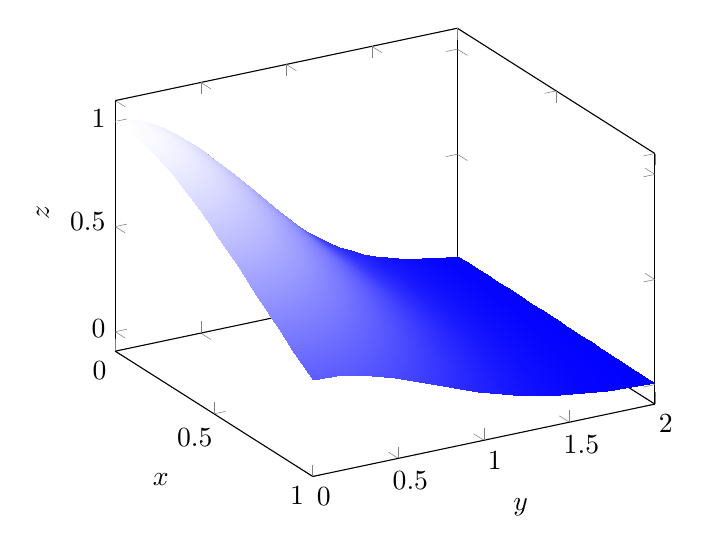
\begin{tikzpicture}
            \begin{axis}[
              view={60}{30}, 
              xlabel={$x$}, ylabel={$y$}, zlabel={$z$},
              domain=0:1, y domain=0:2,
              samples=30,
              colormap/viridis,
              mesh/interior colormap={bluewhite}{color=(blue) color=(white)},
              ]
              \addplot3[surf, shader=interp] 
              {exp(-x^2 - y^2)};
            \end{axis}
          \end{tikzpicture}       
    \end{center}
    b) \\
    It is because $e^{-x^{2}y^{2} = e^{x^{2}} \cdot e^{y^{2}}}$ and the bounds of y are independent of x, so that allows $e^{-x^{2}}$ to be treated as a constant when
    integrating with respect to y and vice versa. \\
    c) 
    \[ \int_0^1 \int_0^2 e^{-x^2 - y^2} \, dy \, dx \approx 0.6588\]
}

\qs{}{
    \begin{enumerate}
        \item[(a)] Find the average value of the function \( f(x, y) = \sin x \cos y \) on the rectangle \( R = [0, \pi] \times [-\pi/2, \pi/2]. \)
        
        \item[(b)] Use symmetry to find the average value of \( f(x, y) = \frac{4 \sin y}{e^{x^2}} - \frac{\cos x}{\ln y} + 3 \) on the region \( R = [2\pi, 4\pi] \times [2\pi, 6\pi]. \) Please explain your answer carefully.
    \end{enumerate}
}

\sol{
    a) 
    \[ f(x,y) = \sin x \cos y \]
    \[ R = [0, \pi ] \times [- \frac{\pi}{2}, \frac{\pi}{2}] \]
    \[ f_{avg} = \frac{1}{A(R)} \iint\limits_{R} f(x,y) dA \]
    \[ A(R) = (\pi - 0 ) \times (\frac{\pi}{2} - -\frac{\pi}{2}) = \pi^{2} \] 
    \[ \frac{1}{\pi^{2}} \int_{0}^{\pi} \int_{-\frac{\pi}{2}}^{\frac{\pi}{2}} \sin x \cos y  \, dy \, dx \] 
    \[ \sin x \int_{-\frac{\pi}{2}}^{\frac{\pi}{2}} \cos y \, dy \]
    \[ \left. (\sin x) \sin y \right|_{\frac{pi}{2}}^{\frac{\pi}{2}} \]  
    \[ (\sin x )\sin\left(\frac{\pi}{2}\right) - (\sin x )\sin\left(\frac{- \pi}{2}\right) = 2 \sin x \] 
    \[ \int_{0}^{\pi} 2 \sin x dx \]
    \[ \left. -2 \cos x \right|_{0}^{\pi} \]
    \[ -\cos \pi - (-2)\cos(0) = 4 \]
    \[ \frac{1}{\pi^{2}} \cdot 4 = \frac{4}{\pi^{2}} \]    
    b) 
    \[ f(x,y) = \frac{4 \sin y}{e^{x^{2}}} - \frac{\cos x}{\ln y} + 3 \]
    \[ R = [2 \pi, 4 \pi ] \times [2\pi, 6 \pi] \]
    \[ f_{avg} = \iint\limits_{R} f(x,y) dA \] 
    \[ A(R) = [4 \pi - 2 \pi ] \times [6\pi - 2 \pi] = 8 \pi^{2} \] 
    \[ \int_{2\pi}^{4 \pi} \int_{2 \pi}^{6 \pi} \frac{4 \sin y}{e^{x^{2}}} - \frac{\cos x}{\ln y }  + 3 \, dy \, dx \]
    \[ \iint\limits_{R} f(x,y) dA  - \iint\limits_{R} \frac{4 \sin y}{e^{x^{2}}} dA - \iint\limits_{R} \frac{\cos x}{\ln y } dA  + \iint\limits_{R} 3 dA\] 
    \[ \int_{2\pi}^{6 \pi} 4 \sin y \, dy = -4\left[ \cos y\right]_{2 \pi}^{6 \pi} = -4(6 \cos \pi - \cos 2 \pi) = -4(1 - 1) = 0 \]
    \[ \iint\limits_{R} f(x,y) \frac{4 \sin y}{e^{x^{2}}} dA = \int_{2 \pi}^{4 \pi} \frac{1}{e^{x^{2}}}dx \times 0 = 0 \]
    \[ \int_{2 \pi}^{4 \pi} {\cos x} dx = \left. \sin x \right|_{2 \pi}^{4 \pi} = sin 4 \pi - \sin 2 \pi = 0 - 0 = 0\] 
    \[ \iint\limits_{R} \frac{\cos x}{\ln y } dA = \int_{2 \pi}^{6 \pi} \frac{1}{\ln y} \times 0 = 0 \] 
    \[ \iint\limits_{R} 3 dA = 3 \times A(R) = 3 \times 8 \pi^{2} = 24 \pi^{2} \]
    \[ \frac{24 \pi^{2}}{8 \pi^{2}} = 3 \]  
}

\qs{}{
    In each part, draw the region \( D \), and evaluate the integral.
    \begin{enumerate}
        \item \( \iint_D \frac{y}{x^5 + 1} \, dA \), where \( D \) is the region \( D = \{(x, y) \mid 0 \leq x \leq 1, \, 0 \leq y \leq x^2 \}. \)
        \item \( \iint_D x^3 \, dA \), where \( D = \{(x, y) \mid 1 \leq x \leq e, \, 0 \leq y \leq \ln x \}. \)
    \end{enumerate}
}

\sol{
    1. 
    \[ \iint_D \frac{y}{x^5 + 1} \, dA  \quad D = \{(x, y) \mid 0 \leq x \leq 1, \, 0 \leq y \leq x^2 \} \]
    \[ \int_{0}^{1} \int_{0}^{x^{2}} \frac{y}{x^{5} + 1} \, dy \, dx \] 
    \[ \frac{1}{x^{5} + 1} \int_{0}^{x^{2}} y dy \]
    \[ \left. \frac{y^{2}}{2}\right|_{0}^{x^{2}} \Rightarrow \frac{\left(x^{2}\right)^{2}}{2} - \frac{0}{2} = \frac{x^{4}}{2} \]  
    \[ \int_{0}^{1} \frac{1}{x^{5} + 1} \times \frac{x^{4}}{2} dx \] 
    \[ x^{5} + 1 = t \quad dt = 5x^{4} dx \] 
    \[ \frac{1}{10} \int_{0}^{1} \frac{1}{t} dt \]
    \[ \left. \frac{1}{10} \ln|t| \right|_{0}^{1} \]
    \[ \left. \frac{1}{10} | x^{5} + 1 | \right|_{0}^{1} \]
    \[ \frac{1}{10} \ln(1^{5} + 1)   - \frac{1}{10}\ln(1) \]
    \[ \frac{1}{10} \ln(2) - \frac{1}{10} \ln(1) = \frac{1}{10} \ln(2) \]  

    \begin{center}
        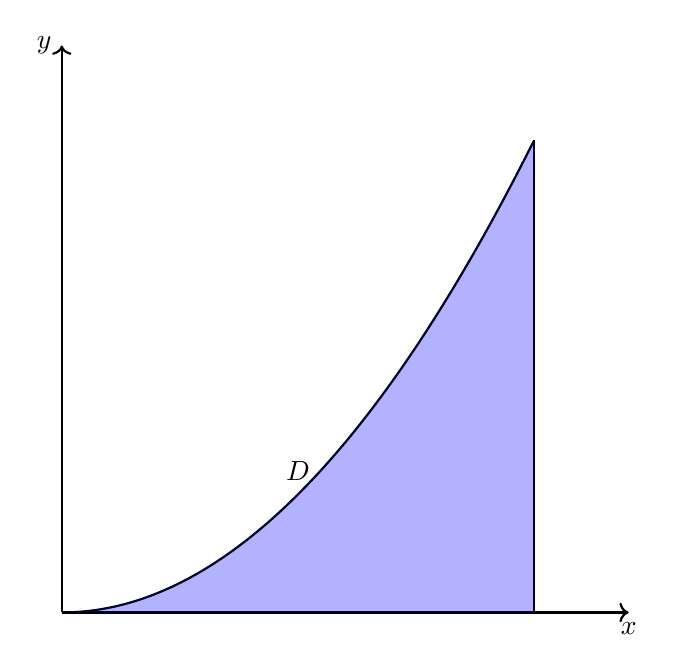
\begin{tikzpicture}[scale=6]
            % Axes
            \draw[thick,->] (0,0) -- (1.2,0) node[anchor=north] {$x$};
            \draw[thick,->] (0,0) -- (0,1.2) node[anchor=east] {$y$};
            % Plot of y = x^2
            \draw[domain=0:1,samples=100,thick] plot (\x,{(\x)^2});
            % Vertical line at x = 1
            \draw[thick] (1,0) -- (1,1);
            % Shading the region D
            \fill[blue,opacity=0.3] (0,0) -- plot[domain=0:1] (\x,{(\x)^2}) -- (1,0) -- cycle;
            % Label the region
            \node at (0.5,0.3) {$D$};
        \end{tikzpicture}
    \end{center}
    2.    
    \[ \iint_D x^3 \, dA  \quad D = \{(x, y) \mid 1 \leq x \leq e, \, 0 \leq y \leq \ln x \} \]
    \[ \int_{1}^{e} \int_{0}^{\ln x} x^{3} \, dy \, dx \]  
    \[ x^{3} \int_{0}^{\ln x} 1 dy \]
    \[ \left. \left(x^{3}\right) y \right|_{0}^{\ln x} \]
    \[ x^{3} \ln x - 0 \]
    \[ uv - \int v \, du \] 
    \[ u = \ln x \quad du = \frac{1}{x}  \, dx \]
    \[ v = \frac{x^{4}}{4} \quad x^{3} dx \]   
    \[ \frac{\ln x \cdot x^{4}}{4} - \int \frac{x^{3}}{4} \, dx \]
    \[ \left[ \frac{\ln x^{4} \cdot x^{4}}{4} - \frac{x^{4}}{16}\right]_{1}^{e} \]
    \[ \left( \frac{\ln e \cdot e^{4} }{4} - \frac{e^{4}}{16} \right) - \left( \frac{\ln 1 \cdot 1^{4}}{4} - \frac{1^{4}}{16}\right)\] 
    \[ \left( \frac{\ln e \cdot e^{4} }{4} \right) - \left( 0 - \frac {1}{16} \right) \]
    \[ \left( \frac{e^{4}}{4} - \frac{e^{4}}{16}\right) + \frac{1}{16} \]   
    \begin{center}
        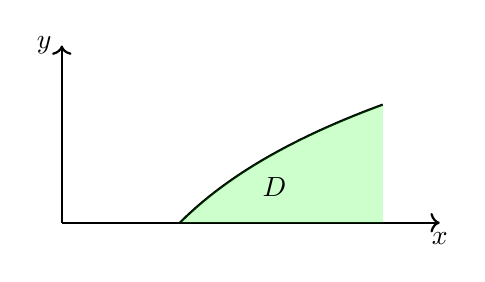
\begin{tikzpicture}[scale=1.5]
            \draw[thick,->] (0,0) -- (3.2,0) node[anchor=north] {$x$};
            \draw[thick,->] (0,0) -- (0,1.5) node[anchor=east] {$y$};
            \draw[domain=1:2.718,samples=100,thick] plot (\x,{ln(\x)});
            \fill[green,opacity=0.2] (1,0) -- plot[domain=1:2.718] (\x,{ln(\x)}) -- (2.718,0) -- cycle;
            \node at (1.8,0.3) {$D$};
        \end{tikzpicture}
    \end{center}

}

\qs{}{
    Draw the region \( D \). Set up the iterated integrals for both orders of integration. 
    Then evaluate the double integral using the easier order and explain why it's easier.
    \[ \iint_D x^2 e^{-xy} \, dA \quad \text{where } D \text{ is bounded by } y = x, \, x = 4, \, \text{and } y = 0. \]
}

\sol{
    \[ \int_{0}^{4} \int_{0}^{x} x^{2}e^{-yx} \, dy \, dx \]
    \[ \int_{0}^{4} \int_{y}^{4} x^{2}e^{-yx} \, dx \, dy \]  
    \[ x^{2} \int_{y}^{4} e^{-yx} dy \] 
    \[ \left. \left( x^{2} \right) \frac{e^{-yx}}{x}  \right|_{0}^{x} \left(x^{2}\right) \frac{e^{-yx}}{x} - \left(x^{2} \right) \frac{e^{-0 \cdot x}}{x} \] 
    \[ xe^{-x^{2}} - x^{2}\cdot \frac{1}{x} \Rightarrow -xe^{-x^{2}} + x \]
    \[ \int_{0}^{4} -xe^{-x^{2}} + x \, dx  \Rightarrow \int_{0}^{4} -xe^{-x^{2}} \, dx \int_{0}^{4} x \, dx \]
    \[ -x^{2} = t \quad -2x = dt \]\
    \[ \int_{0}^{4} \frac{1}{2} e^{t} \, dt \Rightarrow \frac{1}{2} \int_{0}^{4} e^{t} \, dt \] 
    \[ \left. \frac{1}{2} e^{t} \right|_{0}^{4} \Rightarrow \left. \frac{1}{2} ^{x^{2}} \right|_{0}^{4} \] 
    \[ \frac{1}{2}e^{-4^{2}} - \frac{1}{2}e^{-0^{2}} \Rightarrow \frac{1}{2}e^{-16} - \frac{1}{2} \] 
    \[ \int_{0}^{4} x \, dx \]
    \[ \left. \frac{x^{2}}{2} \right|_{0}^{4} \] 
    \[ \frac{4^{2}}{2} - \frac{0^{2}}{2} = \frac{16}{2} = 8 \]
    \[ \int_{0}^{4} -xe^{-x^{2}} + x \, dx  = \frac{1}{2}e^{-16} + \frac{15}{2}\]      

}

\qs{}{
    \begin{enumerate}
        \item[(a)] Find the volume of the solid in the first octant enclosed by the parabolic cylinder \( y = 1 - x^2 \) and the planes \( z = 2 - y \) and \( z = y \).
        
        \item[(b)] Sketch the solid whose volume is given by the iterated integral 
        \[ \int_0^1 \int_0^{1-x} (2 - y^2) \, dy \, dx. \]
    \end{enumerate}
}

\sol{
    \[ y = - x^{2} \quad z = 2 - y \quad z = y \]
    \[ x,y,z \geq 0 \]
    \[ 2 - y = y \Rightarrow 2y = 2 \Rightarrow y = 1 \Rightarrow 0 \leq y \leq 1 - x^{2} \]
    \[ \text{height } = (2 -y) - y \Rightarrow 2 - 2y \]
    \[ V = \int_{0}^{1} \int_{0}^{1-x^{2}} 2 - 2y \, dy \, dx \]
    \[ \int_{0}^{1-x^{2}} 2 - 2y \, dy \]
    \[ \left. 2y - y^{2} \right|_{0}^{1-x^{2}} \]
    \[ 2\left(1-x^{2}\right) - \left(1-x^{2} \right) - 2(0) - (0)^{2} \] 
    \[ 2 - 2x^{2} - 1 + 2x^{2} - x^{4} \]
    \[ 1 - x^{4} \]
    \[ \int_{0}^{1} 1- x^{4} dx \]
    \[ \left. x - \frac{x^{5}}{5} \right|_{0}^{1} \]
    \[ 1 - \frac{1^{5}}{5} - 0 - \frac{0^{5}}{5} \]
    \[ 1 - \frac{1}{5} = \frac{4}{5} \]            
}

\qs{}{
    Sketch the region of integration and change the order of integration.
    \begin{enumerate}
        \item \( \int_0^1 \int_{4x}^4 f(x, y) \, dy \, dx \)
        \item \( \int_0^3 \int_{0}^{\sqrt{9 - y}} f(x, y) \, dx \, dy \)
        \item \( \int_0^4 \int_0^{\ln 2x} f(x, y) \, dy \, dx \)
    \end{enumerate}
}

\sol{\\
    a) 
    \[ \int_{0}^{1} \int_{4x}^{4} f(x,y) \, dy \, dx \]
    \[ \iint\limits_{D} f(x,y) dA \]
    \[ D = \{ (x,y)| 0 \leq x \leq 1, 4x \leq y \leq 4 \} \]
    \[ D = \{ (x,y) | 0 \leq y \leq 4 , 0 \leq x \leq \frac{1}{4} y \} \]\
    \[ \iint_{D} f(x,y) dA = \int_{0}^{4}\int_{0}^{\frac{1}{4}y} f(x,y) \, dx \, dy \]
    b)     
    \[ \int_{0}^{3} \int_{0}^{\sqrt{9-y}} f(x,y) \, dx \, dy \]  
    \[ \iint\limits_{D} f(x,y) dA \]
    \[ D = \{ (x,y)| 0 \leq x \leq \sqrt{9 - y}, 0 \leq y \leq 3 \} \]
    \[ x = \sqrt{9 -y} \quad x^{2} - 9 = - y \quad -x^{2} + 9 = y \]
    \[ -x^{2} + 9 = 3 \quad -x^{2} = - 6 \Rightarrow x^{2} = 6 \Rightarrow x = \sqrt{6} \]  
    \[ D = \{ (x,y)| 0 \leq y \leq -x^{2} + 9, \sqrt{6} \leq x \leq 3 \} \]
    \[ \int_{\sqrt{6}}^{3} \int_{0}^{-x^{2} + 9} f(x,y) \, dy \, dx  \]  
    c) 
    \[ \int_{0}^{4} \int_{0}^{ln 2x} \]
    \[ \iint\limits_{D} f(x,y) dA \quad D = \{ 0 \leq x \leq 4, 0 \leq y \leq ln x \} \]
    \[ y = ln 2x \Rightarrow y = ln 2(4) \Rightarrow y = ln 8 \Rightarrow 0 = ln 2x \Rightarrow ln 1 = \ln 2x 2x \Rightarrow x = \frac{1}{2} \] 
    \[ \iint\limits_{D} f(x,y) dA \quad D = \{ (x,y)| 0 \leq y \leq \ln 8 , \, \frac{1}{2} \leq x \leq \frac{e^{y}}{2} \} \]
    \[ \int_{0}^{\ln 8 } \int_{\frac{1}{2}}^{\frac{e^{y}}{2}}f(x,y) \, dx \, dy \]      
}

\qs{}{
    Evaluate the integral 
    \[ \int_0^1 \int_x^1 e^\frac{x}{y} \, dy \, dx \]
    by reversing the order of integration.
}

\sol{
    \[ \] 
}

\qs{}{
    Evaluate the given integral by converting to polar coordinates. Be sure to draw the region of integration in each part.
    \begin{enumerate}
        \item \( \iint_R (x + y) \, dA \), where \( R \) is the region that lies to the left of the \( y \)-axis between the circles \( x^2 + y^2 = 1 \) and \( x^2 + y^2 = 4 \).
        \item \( \iint_R y e^x \, dA \), where \( R \) is the region in the first quadrant enclosed by the circle \( x^2 + y^2 = 25 \).
    \end{enumerate}
}

\sol{
    a) 
    \[ x \leq 0 \quad x + y^{2} = 1 \quad x^{2} + y^{2} = 4 \]
    \[ x = r \cos \theta \quad y = r \sin \theta \quad dA = r dr \, d \theta \]
    \[ R: 1 \leq r \leq 2 \]
    \[ x + y = r \cos \theta + r \sin \theta \Rightarrow r ( \cos \theta \sin \theta ) \]
    \[ \int_{\frac{\pi}{2}}^{\frac{\pi}{2}} \int_{1}^{2} r(\cos \theta \sin \theta ) r \, dr \, d\theta\] 
    \[ \cos \theta + \sin \theta \int_{1}^{2} r^{2} dr \]
    \[ \left. \frac{r^{3}}{3} \right|_{1}^{2} \]
    \[ \frac{2^{3}}{3} - \frac{1}{3} =  \frac{7}{3} \]
    \[ \frac{7}{3} \int_{\frac{\pi}{2}}^{\frac{3 \pi}{2}} \cos \theta + \sin \theta \, d \theta \]
    \[ \left. \frac{7}{3} \sin \theta \right|_{\frac{\pi}{2}}^{\frac{3 \pi}{2}} - \left. \frac{7}{3} \cos \theta \right|_{\frac{\pi}{2}}^{\frac{3 \pi }{2}} \]   
    \[ \frac{7}{3}(-1) - \frac{7}{3}(1) = -\frac{14}{3} \]
    \[ -\frac{7}{3} \cos \frac{3 \pi}{2} + \frac{7}{3} \cos \frac{\pi}{2} \]
    \[ - \frac{7}{3} (0) + \frac{7}{3} = 0 \]
    \[ - \frac{14}{2}\]
    b)           
    \[ \iint\limits_{R} ye^{x} dA \]
    \[ x = r \cos \theta \quad y = r \sin \theta \quad x^{2} + y^{2} = 25 \]
    \[ \text{ 1st quadrant } \quad 0 \leq \theta \leq \frac{\pi}{2} \]
    \[ ye^{x} \Rightarrow r \sin \theta e ^{r \cos \theta } \]
    \[ dA = r \, dr \, d\theta \]
    \[ \int_{0}^{\frac{\pi}{2}} \int_{0}^{5} r \sin \theta e^{r \cos \theta }\] 
    \[  I(\theta) = \int_{0}^{5} r^{2} \sin \theta \, e^{r \cos \theta} \, dr \] 
    \[ \frac{\partial}{\partial \theta} e^{r \cos \theta} = -r \sin \theta \, e^{r \cos \theta} \]
    \[ r \sin \theta e^{r \cos \theta} = - \frac{\partial}{\partial \theta} e^{r \cos \theta} \]
    \[ I = \int_{0}^{\frac{\pi}{2}} \int_{0}^{5} - r \frac{\partial}{\partial \theta} e^{r \cos \theta} \, dr \, d\theta \]
    \[ I = - \int_{0}^{5} r \left( \int_{0}^{\frac{\pi}{2}} \frac{\partial }{\partial \theta} e^{r \cos \theta} \, d\theta \right) dr \]
    \[ \int_{0}^{\frac{\pi}{2}} \frac{\partial}{\partial \theta} e^{r \cos } \, d \theta = \left. e^{r \cos \frac{\pi}{2}} \right|_{0}^{\frac{\pi}{2}} \] 
    \[ e^{r \cos \frac{\pi}{2}} - e^{r \cos \theta} = e^{r \cdot 0} - e^{r \cdot 1} = 1 - e^{r} \] 
    \[ I = \int_{0}^{5} re^{r} dr - \int_{0}^{3} r dr \]
    \[ u = r \quad du = dr \quad v = e^{r} \quad dv = e^{r} dr \]
    \[ \int_{0}^{5} re^{r} dr = re^{r} - \int_{0}^{5} e^{r} dr = re^{r} -e^{r} + K \]
    \[ \int_{0}^{5} re^{r} dr = \left[ re^{r} - e^{r} \right]_{0}^{5} = \left( 5e^{5} - e^{5} \right) - (0 - e^{0}) = 4e^{5} + 1 \]
    \[ \int_{0}^{5} r dr = \left. \frac{1}{2}r^{2} \right|_{0}^{5} = \frac{1}{2} (25 - 0 ) = \frac{25}{2} \] \
    \[ I = (4e^{5} + 1) - \frac{25}{2} = 4e^{5} - 11.5  \]              
}

\qs{}{
    Use polar coordinates to find the volume of the given solid.
    \begin{enumerate}
        \item[(a)] Inside the sphere \( x^2 + y^2 + z^2 = 4 \) and outside the cylinder \( x^2 + y^2 = 1 \).
        \item[(b)] Bounded by the paraboloids \( z = 3x^2 + 3y^2 \) and \( z = 4 - x^2 - y^2 \).
    \end{enumerate}
}

\sol{
    a) 
    \[ x^{2} + y^{2} + z^{2} = 4 \quad  x^{2} + y^{1} = 1  \] 
    \[ x = r \cos \theta \quad y = r \sin \theta \quad 0 \leq \theta \leq 2 \pi \]
    \[ r^{2} + z^{2} = 4 \quad x^{2} + y^{2} = 1 \Rightarrow r^{2} = 1 \Rightarrow r = 1 \]
    \[ r^{2} + z^{2} = 4 \Rightarrow r^{2} = 4 - z^{2} \Rightarrow r = \sqrt{4 - z^{2}} \]
    \[ V = \iint\limits_{D} \left[ z_{\text{upper}} - z_{\text{lower}} \right]\]
    \[ V = \int_{0}^{2\pi}\int_{1}^{2}   r \sqrt{4 - r^{2} - \left( - \sqrt{4 - r^{2}} \right)}  r \, dr \, d \theta \]
    \[ V = 2 \int_{0}^{2 \pi} \int_{1}^{2} \sqrt{4 - r^{2}} \, dr \, d \theta \]
    \[ 4 - r^{2} = t \quad -2r = dt \]
    \[ - \int_{1}^{2} \frac{1}{2} \sqrt{t} dt \Rightarrow - \frac{1}{2} \int_{1}^{2} \sqrt{t} dt = \left. - \frac{1}{2} \cdot \frac{2t\sqrt{t}}{3} \right|_{1}^{2} \]
    \[ \left. - \frac{1}{2} \cdot \frac{2(4-r^{2})\sqrt{4-r^{2}}}{3} \right|_{1}^{2} \left( - \frac{1}{2} \cdot \frac{2(4-2^{2})\sqrt{4-2^{2}}}{3} \right) - \left( - \frac{1}{2} \cdot \frac{2(4-1^{2})\sqrt{4-1^{2}}}{3}\right) \]    
    \[ V = 2 \left( \int_{2}^{2\pi} d \theta \right) \left(\int_{1}^{2} r\sqrt{4-r^{2}} dr \right)\]   
    \[ \int_{0}^{2 \pi} d \theta = 2 \pi \quad V = 2 \cdot 2 \pi \cdot \int_{1}^{2} r \sqrt{4-r^{2}} dr = 4 \pi \int_{1}^{2} r \sqrt{4 - r^{2}} dr \]
    \[ - \left(- \frac{1}{2} \cdot \frac{2(3)\sqrt{3}}{3} \right) \Rightarrow \left( \frac{1}{2} \sqrt{3} \right)  \Rightarrow - (- \sqrt{3}) \]
    \[ 4 \pi \sqrt{3} \]  
    b) 
    \[ z = 3x^{2} 3y^{2} = 3\left(x^{2} + y^{2} \right) = 3\left(x^{2} + y^{2}\right) = 3r^{2} \]
    \[ z = 4 - x^{2} - y^{2} = 4 - r^{2} \]
    \[ 3r^{2} = 4 - r^{2} \]
    \[ 4r^{2} = 4 \Rightarrow r = 1 \]
    \[ \int_{0}^{2\pi} \int_{0}^{1} \left( 4 - r^{2} - 3r^{2} \right)r \, dr \, d\theta \]
    \[ \int_{0}^{2\pi} \int_{0}^{1} \left( 4 - 4r^2\right)r \, dr \, d\theta \]
    \[ \left.  2r - r^{4}\right|_{0}^{1} \, d \theta \Rightarrow \left(2(1)^{2} - 1 \right) - 0 \]
    \[ \int_{0}^{2 \pi} 1 \, d\theta \] 
    \[ \left. \theta \right|_{0}^{2\pi} = 2\pi \]             
}

\qs{}{
    Evaluate the iterated integral 
    \[ \int_0^b \int_{-\sqrt{b^2 - y^2}}^0 x^2 y \, dx \, dy \]
    by converting to polar coordinates.
}

\sol{   
    \[ \int_{0}^{b} \int_{- \sqrt{b^{2} - y^{2}}}^{0} x^{2}y \, dx \, dy\]
    \[ y = 0 \quad \text{to } \quad y = b \] 
    \[ x = - \sqrt{b^{2} - y^{2} } \text{to } \quad \text{to } {x = 0 } \]
    \[ \text{left half of } x^{2}+y^{2} = b^{2} \]
    \[ x = r \cos \theta \quad y = r \sin \theta \quad 0 \leq r \leq b \quad \frac{\pi}{2} \leq \theta \pi \] 
    \[ x^{y} = (r \cos \theta )^{2} (r \sin \theta) = r^{3} \cos \theta \sin \theta \]
    \[ \int_{\frac{\pi}{2}}^{\pi} \int_{0}^{b} \left(r^{3} \cos^{2} \theta \sin \theta \right) r \, dr \, d\theta \]
    \[ \int_{\frac{\pi}{2}}^{\pi} \int_{0}^{b} r^{4} \cos^{2} \theta \sin \theta \, d\theta \, dr \]
    \[ \cos^{2}\theta \sin \theta \int_{0}^{b} r^{4} \, dr \] 
    \[ \left. \cos^{2}\theta \sin \theta \frac{r^{5}}{5} \right|_{0}^{b} \]
    \[ \cos^{2}\theta \sin \theta \frac{b^{5}}{5} - 0 \]     
    \[ \int_{\frac{\pi}{2}}^{\pi} \frac{b^{5}}{5} \cos^{2}\sin \theta \, d \theta \]
    \[ \frac{b^{5}}{5} int_{\frac{\pi}{2}}^{\pi} \cos^{2}\sin\theta \]
    \[ \left. \frac{b^{5}}{5} \frac{\cos^{3}\theta}{3} \right|_{\frac{\pi}{2}}^{\pi} \]
    \[ \left(\frac{b^{5}}{5}\right)\left(\frac{\cos^{3} \frac{\pi}{2}}{3}\right) - \left(\frac{b^{5}}{5}\right)\left(\frac{\cos^{3} \pi }{3}\right)\] 
    \[ 0 - \frac{b^{5}}{5} \cdot \frac{-1}{3} \]
    \[ \frac{b^{5}}{15}\]        
}

\qs{}{
    Let \( D \) be the disk with center at the origin and radius \( a \).
    \begin{enumerate}
        \item[(a)] Use your intuition: what do you expect is the average distance from points on the disk to the origin?
        \begin{itemize}
            \item less than \( a/2 \)
            \item \( a/2 \)
            \item between \( a/2 \) and \( a \)
            \item more than \( a \)
        \end{itemize}
        Give an intuitive explanation of your answer.

        \item[(b)] What is the average distance from points in the disk to the origin?
    \end{enumerate}
}

\sol{
    The area of the disk should be greater on the interval of $\left[ \frac{a}{2}, a \right] $ than from $\left[0, \frac{a}{2} \right]$ which means 
    there are more points on the interval of  $\left[ \frac{a}{2}, a \right] $ meaning hte average distance is on this interval. 
    \\
    b) \\
    \[ D = \frac{1}{A} \iint\limits_{A} d \, \, da \]
    \[ D = \frac{1}{A} \int_{0}^{2\pi}\int_{0}^{a} r \cdot r \, dr \, d\theta \]
    \[ \left. \frac{r^{3}}{3}\right|_{0}^{a} \Rightarrow \frac{a^{3}}{3} - 0  = \frac{a^{3}}{3} \]
    \[ A = a^{2}\pi \]
    \[ \frac{1}{a^{2} \pi} \int_{0}^{2\pi} \frac{a^{3}}{3} \, d\theta \]
    \[ \left. \frac{1}{a^{2} \pi} \left(\frac{a^{3}}{3}\right) \right|_{0}^{2\pi} \]
    \[ \frac{2a}{3} \]       
}

\end{document}
